The above equation can be expressed as
\begin{align}
        \vec{x}^{T}\vec{Vx} + 2\vec{u}^{T}\vec{x} + f=0   \label{eq:solutions/13/12/eq2}
\end{align}
where
\begin{align}
	\vec{V}=\vec{V}^T &= \myvec{12 & \frac{7}{2} \\ \frac{7}{2} & -10} \\
	\vec{u} &= \myvec{\frac{13}{2} \\ \frac{45}{2}} \\
	 f=-35
\end{align}	
	(\ref{eq:solutions/13/12/eq2}) represents a pair of straight lines if
\begin{align}
	&\mydet{\vec{V} & \vec{u} \\ \vec{u}^T & f} = 0     \label{eq:solutions/13/12/eq5} \\
	\mydet{\vec{V} & \vec{u} \\ \vec{u}^T & f} 
		&= \mydet{12 & \frac{7}{2}  & \frac{13}{2} \\ 
	        \frac{7}{2} & -10 & \frac{45}{2}     \\
	       \frac{13}{2} & \frac{45}{2} & -35 }  \\
	       		\nonumber \\
	\implies \ 12\mydet{-10 & \frac{45}{2} \\ \frac{45}{2} & -35} 
		& -\frac{7}{2}\mydet{\frac{7}{2} & \frac{45}{2} \\ \frac{13}{2} & -35} 
		+\frac{13}{2}\mydet{\frac{7}{2} & -10 \\ \frac{13}{2} & \frac{45}{2}} = 0 \label{eq:solutions/13/12/eq10}\\
\end{align}
The lines intercept if
\begin{align}
        \mydet{\vec{V}} < 0 \\
 	\mydet{\vec{V}}=-\frac{529}{4} < 0 \label{eq:solutions/13/12/eq11}
\end{align}
From (\ref{eq:solutions/13/12/eq10}) and (\ref{eq:solutions/13/12/eq11}) it can be concluded that the given equation represents a pair of intersecting lines.
Let the equations of lines be
\begin{align}
	\vec{n_1}^T \vec{x}=c_1 \\
	\vec{n_2}^T \vec{x}=c_2 
\end{align}
Since (\ref{eq:solutions/13/12/eq2}) represents a pair of straight lines it must satisfy
\begin{align}
	(\vec{n_1}^T \vec{x} - c_1)(\vec{n_1}^T \vec{x} - c_1) =
        \vec{x}^{T}\vec{Vx} + 2\vec{u}^{T}\vec{x} + f=0
\end{align}
where
\begin{align}
	\vec{n_1}*\vec{n_2}=\myvec{a\\2b\\c}=\myvec{12\\7\\-10} \label{eq:solutions/13/12/eq6} \\ 
	c_2\vec{n_1}+c_1\vec{n_2}=-2\vec{u} \label{eq:solutions/13/12/eq9}\\
	c_1c_2=f
\end{align}
Slopes of the lines can be obtained by solving 
\begin{align}
	cm^2+2bm+a=0 \\
	-10m^2+7m+12=0 \\
	\implies m_1 = \frac{-4}{5}, m_2 = \frac{3}{2}
\end{align}
The normal vectors can be expressed in terms of corresponding slopes of lines as
\begin{align}
	\vec{n}=k\myvec{-m\\1} \\
	\implies
	\vec{n_1}=k_1\myvec{\frac{4}{5} \\ 1}  \label{eq:solutions/13/12/eq7} \\
	\vec{n_2}=k_2\myvec{-\frac{3}{2} \\ 1}  \label{eq:solutions/13/12/eq8}
\end{align}
Substituing (\ref{eq:solutions/13/12/eq7}) and (\ref{eq:solutions/13/12/eq8}) in (\ref{eq:solutions/13/12/eq6}) we get
\begin{align}
	k_1k_2=-10
\end{align}
Assuming $ k_1=5$ and $k_2 =-2$
\begin{align}
	\vec{n_1}=\myvec{4\\5}, \vec{n_2}=\myvec{3\\-2}
\end{align}
Verification using Toeplitz matrix
\begin{align}
\vec{n_1}*\vec{n_2}=\myvec{4 & 0 \\ 5 & 4 \\0 & 5}\myvec{3\\-2}=\myvec{12\\7\\-10}
\end{align}
From (\ref{eq:solutions/13/12/eq9}) we have
\begin{align}
	c_2\myvec{4\\5}+c_1\myvec{3\\-2}=\myvec{-13\\-45}
\end{align}
Solving the augmented matrix
\begin{align}
	\myvec{4 & 3 & -13 \\ 5 & -2 & -45}
	\xleftrightarrow[]{R_2 \leftarrow 4R_2-5R_1}
	\myvec{4 & 3 & -13 \\ 0 & -23 & -115}\\
	\xleftrightarrow[]{R_2 \leftarrow -\frac{R_2}{23}}
        \myvec{4 & 3 & -13 \\ 0 & 1 & 5}
        \xleftrightarrow[]{R_1 \leftarrow R_1-3R_2}
	\myvec{4 & 0 & -28 \\ 0 & 1 & 5}\\
	\xleftrightarrow[]{R_1 \leftarrow \frac{R_1}{4}}
        \myvec{1 & 0 & -7 \\ 0 & 1 & 5} \\
	\implies \quad c_1 =-7, \ c_2 =5
\end{align}
Thus the equation of lines are
\begin{align}
	\myvec{4 & 5}\vec{x} = 5 \\
	\myvec{3 & -2}\vec{x} = -7 
\end{align}
The angle between the lines can be expressed interms of normal vectors 
\begin{align}
	\vec{n_1}=\myvec{4\\5} , \quad \vec{n_2}=\myvec{3\\-2}
\end{align}
as
\begin{align}
	\cos\theta=\frac{\vec{n_1}^T\vec{n_2}}{\norm{\vec{n_1}}\norm{\vec{n_2}}} \\
				\nonumber \\
	\implies \quad \theta=\cos^{-1}({\frac{2}{\sqrt{533}}}) = \tan^{-1}(\frac{23}{2})
\end{align}
\begin{figure}[!h]
	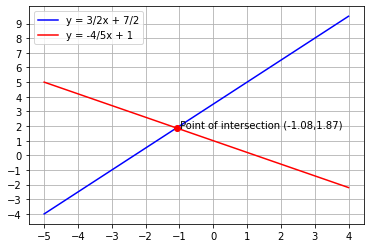
\includegraphics[width=\columnwidth]{./solutions/13/12/lines.png}
	\caption{} \label{eq:solutions/13/12/linefig1}
\end{figure}
